\subsubsection{Drone table}
Tabellen indeholder alle droner som er oprettet i systemet. Brugeren kan oprette nye droner
\vspace{-5pt}
\begin{figure}[H]
	\centering
	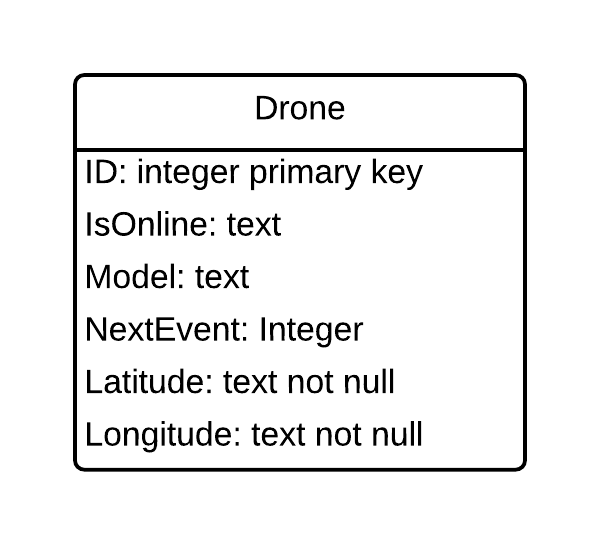
\includegraphics[width=0.5\textwidth]{Billeder/database/DroneTable.png}
	\vspace{-5pt}
	\caption{Drone table}
	\label{fig:drone_table}
\end{figure}

\begin{table}[H]
\begin{tabular}{| p{3cm}| p{11.5cm}|}
\hline

Formål	 							& Holde data om billeder i systemet og selve billederne.\\\hline
Forbindelser						& Tabellen har en foreing key til event tabllen.\\\hline
Attributter						& \begin{itemize}
												\item ID: Primary key.
												\item IsOnline: Status for dronen: Boolean værdig
												\item Model: Modeltype: Text field: Max length 50 char
												\item NextEvent: Events for dronen: Integer field
												\item Latitude: Dronens GPS lokation: Max length 100 char  
												\item Longitude: Dronens GPS lokation: Max length 100 char
											\end{itemize} \\\hline 
\end{tabular}
\caption{Drone table}
\label{tab:drone_table}
\end{table}